% vim: set spell spelllang=es syntax=tex :

\documentclass[11pt,a4paper,spanish]{beamer}

\usepackage[spanish]{babel}

\usepackage[utf8]{inputenc}

\usepackage{graphicx}

\usepackage{subcaption} %Para Subfigure

\usepackage{caption} %Para captions en las figuras sin prefijo

\usepackage{upquote} % Para comillas rectas en verbatim
\usepackage{fancyvrb}
\usepackage{inconsolata}
\usepackage{lmodern}
\usepackage{pmboxdraw} % Para poder usar la salida del comando tree
\usepackage{ccicons}

\usepackage{url}

\usepackage{babelbib}

\usefonttheme{serif}

\setlength{\parskip}{1.5mm}
\newcommand{\cw}[1]{\mbox{\texttt{\textcolor{blue}{#1}}}}
\newcommand{\dq}[0]{\Verb+"+}
\newcommand{\sq}[0]{\textquotesingle}

\usetheme{Rochester}
\usecolortheme{whale}

%\usetheme{Warsaw}

\beamertemplatenavigationsymbolsempty

\setbeamertemplate{background canvas}{
    \raisebox{-0.99\paperheight}[0pt][0pt]{
        \makebox[\paperwidth]{
            \null
            \hspace{-1em}
            
\includegraphics[width=0.09\paperwidth]{logos/fai.pdf}
            \hspace{0.8\paperwidth}
            %\hfill
            \hspace{-1em}
            
\includegraphics[width=0.09\paperwidth]{logos/uncoma.pdf}
            }
    }
}

\title{Editores de texto \texttt{Vi} y \texttt{Vim}}

\author{}

\date{}

\defbeamertemplate{footline}{centered page number}
{
    \hspace*{\fill}
    \usebeamercolor[fg]{blue}
    \usebeamerfont{page number in head/foot}
    \insertpagenumber\,/\,\insertpresentationendpage
    \hspace*{\fill}\vskip2pt
}
\setbeamertemplate{footline}[centered page number]

\begin{document}

\begin{frame}[noframenumbering]

    \maketitle
    \centering
    \vspace{-8em}~
    \begin{figure}
    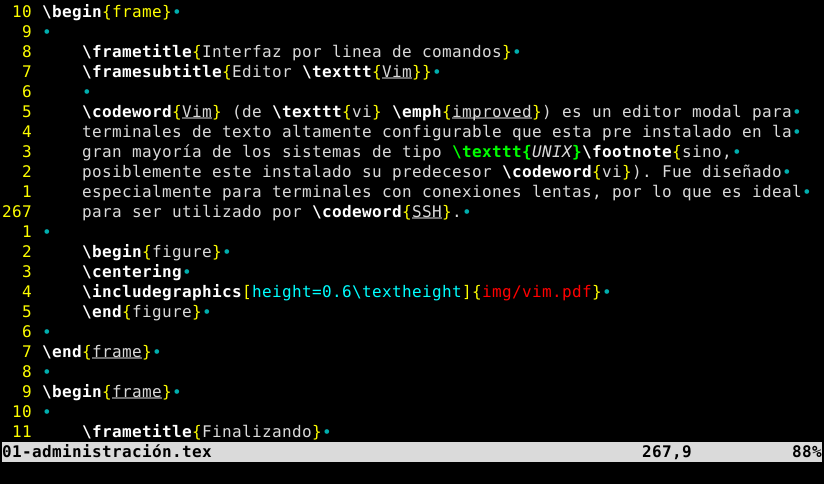
\includegraphics[height=0.55\textheight]{img/vim.pdf}
        \captionsetup{textfont=tiny,labelformat=empty}
        \caption{}
    \end{figure}

\end{frame}

\begin{frame}[label=temario]

    \frametitle{Temario}

\begin{itemize}

    \item Breve historia de \cw{Vi} y \cw{Vim}.
    \item Modos principales.
    \item Movimientos básicos.
    \item Sistema de \cw{[N]}\emph{verbo}\cw{[M]}\textbf{objeto}.
    \item Comandos básicos.

\end{itemize}

\end{frame}

\begin{frame}

    \frametitle{Breve historia de \texttt{Vi} y \texttt{Vim}}
    \framesubtitle{\emph{\texttt{ed} is the standard text editor}}
    
    \cw{ed} es un editor de texto basado en lineas, pensado para terminales
    teletipo\footnote{Ver \url{https://www.youtube.com/watch?v=-Ul-f3hPJQM}}.
    Desarrollado en 1969 por \emph{Ken Thompson}, fue uno de los primeros
    programas de \cw{UNIX}.

    \begin{figure}
    \centering
    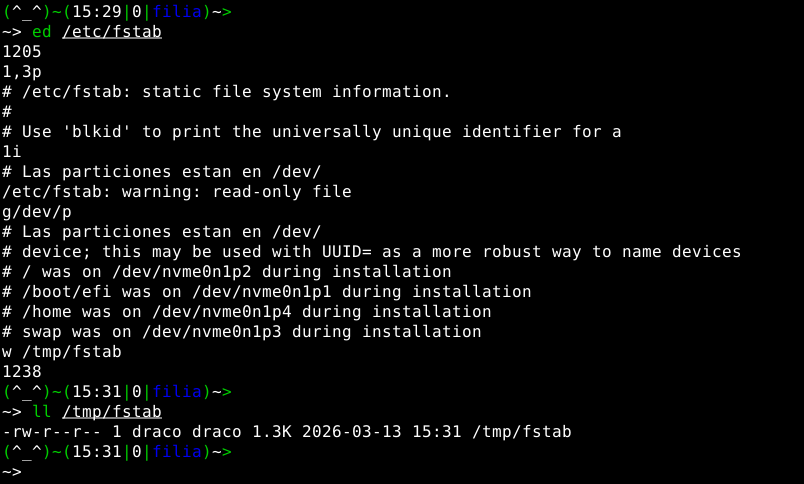
\includegraphics[height=0.5\textheight]{img/ed.pdf}
    \end{figure}

\end{frame}

\begin{frame}

    \frametitle{Breve historia de \texttt{Vi} y \texttt{Vim}}
    \framesubtitle{\texttt{ex} y \texttt{vi}}
    
    En 1976 \emph{bill Joy} comenzó a trabajar sobre \cw{ed} para hacerlo más
    apto para ``\emph{mortales}''. En 1978 se incluyo \cw{ex} en \cw{BSD
    UNIX}, al que se le agrego un modo \emph{visual}. En 1979 se agrego se
    agrego un link el cual permitía iniciar a \cw{ex} en modo visual al
    ejecutarlo como \cw{vi}.

    \begin{figure}
    \centering
    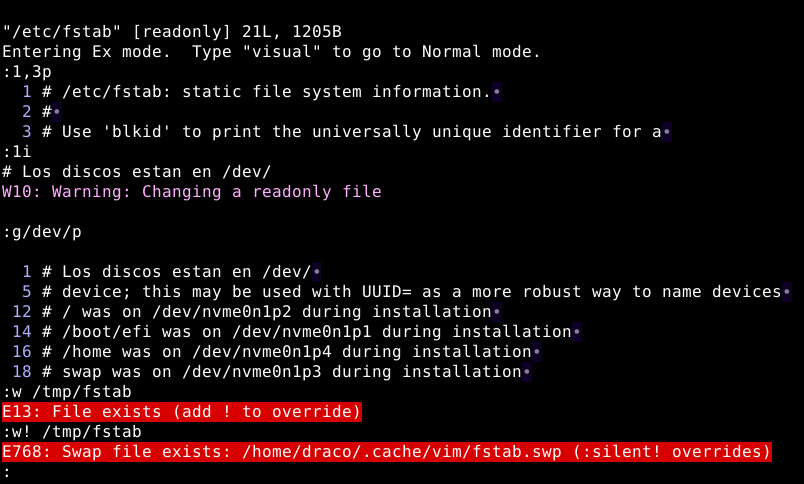
\includegraphics[height=0.5\textheight]{img/ex.pdf}
    \end{figure}

\end{frame}

\begin{frame}

    \frametitle{Breve historia de \texttt{Vi} y \texttt{Vim}}
    \framesubtitle{Editor \texttt{Vim} (\texttt{vi} \emph{improved})}
    
    \cw{Vim} fue desarrollado en 1992 por \emph{Bram Moolenaar} para la
    \emph{Amiga}. Actualmente se encuentra disponible para gran cantidad de
    sistemas.

    Es un editor modal, altamente configurable, y que esta pre instalado en la
    gran mayoría de los sistemas de tipo \cw{UNIX}.

    \begin{figure}
    \centering
    
\includegraphics[height=0.25\textheight]{img/vimlogo.pdf}
        \captionsetup{textfont=tiny,labelformat=empty}
        \caption{Logo de \cw{Vim}\cite{vimlogo}}
    \end{figure}

\end{frame}

\begin{frame}

    \frametitle{Modos principales de \texttt{Vim}}

    \begin{itemize}
        \item \cw{Modo normal:} es el modo en el que inicia \cw{Vim}. En este
            modo, cada tecla tiene un comando asociado que se ejecutara al
            presionarla. Por ejemplo: \cw{w} mueve el cursor hasta la
            siguiente palabra, \cw{dd} remueve la linea actual del documento,
            y guarda una copia en el registro \cw{\dq{}}. Se puede entrar en este
            modo con la tecla \cw{Escape}.
        \item \cw{Modo inserción:} se ingresa desde \cw{modo normal} al presionar
            la teclas \cw{i}, \cw{R}, \cw{I}, entre otras. Permite ingresar
            texto (es decir, no se ejecutan funciones especiales al presionar
            una tecla, sino que simplemente se ingresa como texto).
        \item \cw{Modo linea de comando:} se ingresa desde \cw{modo normal} al
            presionar la tecla \cw{:}. Permite ingresar comandos similares a
            los de \cw{ex}.
    \end{itemize}

\end{frame}

\begin{frame}

    \frametitle{Movimientos básicos}

    En modo normal, con pocas teclas podemos movernos rápidamente dentro de un
    documento:

    \begin{itemize}
        \item \cw{h j k l} son las teclas preferidas para moverse un caracter
            a la izquierda, hacia las lineas de arriba y abajo, o un caracter
            a la derecha.
        \item \cw{gg G gi} nos permiten movernos al inicio y final del
            documento, o a la posición donde se inserto texto por última vez
            (y se cambia a \cw{modo inserción}).
        \item \cw{w e b} permiten movernos al comienzo o final de la próxima
            palabra, o una palabra hacia atrás.
        \item \cw{( )} permiten movernos una oración hacia atrás o adelante.
        \item \cw{\{ \}} permiten movernos un párrafo hacia atrás o adelante.
        \item \cw{/ n} permiten buscar en el documento, y luego movernos entre
            ocurrencias.
    \end{itemize}

\end{frame}

\begin{frame}

    \frametitle{Sistema de \texttt{[N]}\emph{verbo}\texttt{[M]}\textbf{objeto}}

    Algunos comandos de \cw{modo normal} necesitan que se especifique un
    objeto sobre el que se quiere aplicar la acción. Por ejemplo, el comando
    \cw{d} permite borrar, si se quiere borrar una palabra una palabra se
    puede pulsar \cw{dw}, si se desea borrar hasta el final del documento se
    puede pulsar \cw{dG}.

    Ademas, se puede agregar números de repeticiones a los comandos o
    movimientos. Si se quiere avanzar 5 oraciones es suficiente con pulsar
    \cw{5(}, y si se quieren eliminar las siguientes 5 se puede pulsar
    \cw{5d(}.

\end{frame}

\begin{frame}

    \frametitle{Comandos básicos}

    \emph{(\cw{+} indica que el comando requiere que se indique una
    dirección)}
    \begin{itemize}
        \item \cw{d+ y+ p} permiten eliminar, copiar o pegar un objeto. Si en
            lugar de una dirección se repite la letra, se aplica sobre toda la
            linea.
        \item \cw{u} permite revertir la última acción\footnote{si por error
            presionan \cw{ctrl-z}, el \cw{vim} se pasara a segundo plano. Para
            volver ejecutar \cw{fg} en la consola}.
        \item \cw{:q :q!} terminan la ejecución. La segunda opción permite
            cerrar aunque haya cambios sin guardar.
        \item \cw{:w} guarda los cambios del archivo actual.
        \item \cw{:help} muestra la ayuda de \cw{Vim}.
    \end{itemize}

\end{frame}

\againframe{temario}

\begin{frame}

\title{¿Consultas?}
\maketitle

\end{frame}

\newcounter{lastPage}
\setcounter{lastPage}{\number\value{page}}

\begin{frame}%[allowframebreaks]

\frametitle{Atribuciones}

\bibliographystyle{abbrv}
\setbeamertemplate{bibliography item}{\insertbiblabel}
\tiny
\bibliography{refimg}
\end{frame}

\setcounter{page}{\number\value{lastPage}}

\end{document}
